
\begin{remark}{7.2.297}\label{rem:7-2-297}
可以仿照 (7.2.135) 定义
\[
\begin{aligned}
(\operatorname{Incl}_s)_{1,\beta_0}\colon
S([0,1]_r\times L'_1)&\longrightarrow
S([0,1]^2\times L'_1),\\
(\operatorname{Incl}_r)_{1,\beta_0}\colon
S([0,1]_s\times L'_1)&\longrightarrow
S([0,1]^2\times L'_1).
\end{aligned}
\]
可选择棱柱剖分，使两个复合
\[
\begin{aligned}
(\operatorname{Incl}_s)_{1,\beta_0}
\circ(\operatorname{Incl}_r)_{1,\beta_0}
&\colon S(L'_1)\longrightarrow
S([0,1]^2\times L'_1),\\
(\operatorname{Incl}_r)_{1,\beta_0}
\circ(\operatorname{Incl}_s)_{1,\beta_0}
&\colon S(L'_1)\longrightarrow
S([0,1]^2\times L'_1)
\end{aligned}
\]
的像均满足 (7.2.289.3)。
因此，可以选其中任一个作为
$(\operatorname{Incl})_{1,\beta_0}$ 的定义。
不过，应注意下式并不成立：
\begin{equation}
(\operatorname{Incl}_r)_{1,\beta_0}
\circ(\operatorname{Incl}_s)_{1,\beta_0}
=(\operatorname{Incl}_s)_{1,\beta_0}
\circ(\operatorname{Incl}_r)_{1,\beta_0}.
\tag{7.2.189bis3}
\end{equation}
例如，取单形
$P=[0,1]\in C(L'_1)$。\translatornote{原书在本例中把
$P$ 所属复形及随后的截面空间写为 $L'$；
但本注所定义的两个包含映射均以 $L'_1$ 为底空间，
这里据其源靶统一补下标。}
分别考察
$(\operatorname{Incl}_s\circ\operatorname{Incl}_r)(P)$
与
$(\operatorname{Incl}_r\circ\operatorname{Incl}_s)(P)$
在
\[
\bigl\{(s,r)\mid s+r=1/4\bigr\}\times L'_1
\]
上的部分。
二者都是矩形，但其单纯剖分不同
（见图~\ref{fig:7-2-17}）。

\par\medskip\noindent\begin{minipage}{\textwidth}
\centering
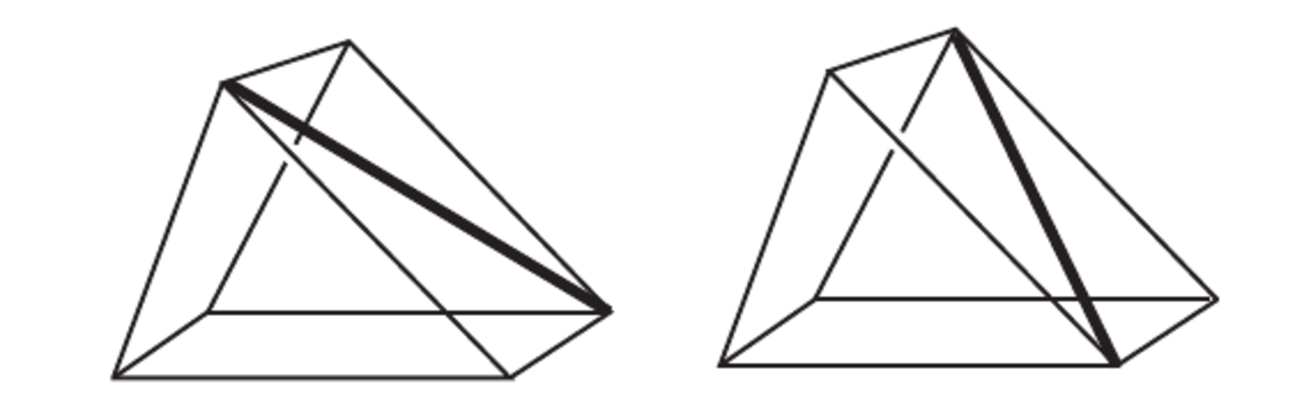
\includegraphics[width=.65\textwidth]{chapters/ch07-transversality/figures/phys-558-figure-7-2-17-math-crop.png}
\par{\renewcommand{\thefigure}{7.2.17}\refstepcounter{figure}
\normalfont\bfseries 图~\thefigure\label{fig:7-2-17}}
\end{minipage}\par\medskip
\end{remark}

至此，我们已完成对 (7.2.280.2) 的讨论。
这实际上是命题~\ref{prop:7-2-275} 证明中
主要的几何部分。
后续部分将处理 $\mathfrak f$ 与
$\mathfrak g$ 的差异；
这种差异源于构造过程中需要多次修改链复形。
遗憾的是，这部分颇具技术性，记号也相当繁重。
